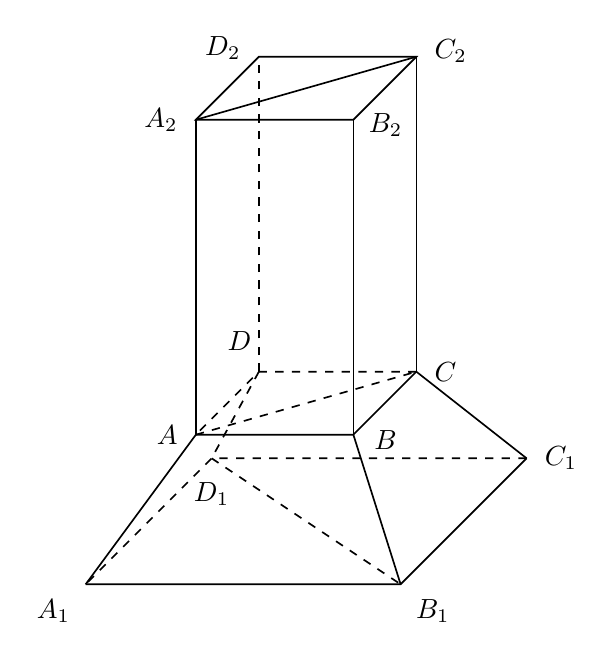
\begin{tikzpicture}[x=1cm,y=1cm,line width=.6pt]
% stacked frustum (bottom) + prism (top); schematic oblique projection
\coordinate (A) at (0,0);
\coordinate (B) at (2,0);
\coordinate (C) at (2.8,0.8);
\coordinate (D) at (0.8,0.8);
\coordinate (A2) at (0,4);
\coordinate (B2) at (2,4);
\coordinate (C2) at (2.8,4.8);
\coordinate (D2) at (0.8,4.8);
\coordinate (A1) at (-1.4000000000,-1.9000000000);
\coordinate (B1) at (2.6000000000,-1.9000000000);
\coordinate (C1) at (4.2000000000,-0.3000000000);
\coordinate (D1) at (0.2000000000,-0.3000000000);
% top prism
\draw (A2)--(B2)--(C2)--(D2)--cycle;
\draw (A)--(A2) (B)--(B2) (C)--(C2);
\draw[dashed] (D)--(D2);
\draw (A2)--(C2);
\draw (A)--(B)--(C);
\draw[dashed] (C)--(D)--(A) (A)--(C);
% bottom frustum
\draw (A)--(A1) (B)--(B1) (C)--(C1);
\draw[dashed] (D)--(D1);
\draw (A1)--(B1)--(C1);
\draw[dashed] (C1)--(D1)--(A1);
\draw[dashed] (D1)--(B1);
% labels offset to avoid strokes
\node[left=3pt] at (A) {$A$};
\node[below right,xshift=4pt,yshift=5pt] at (B) {$B$};
\node[right,xshift=3pt] at (C) {$C$};
\node[above=3pt,xshift=-7pt,yshift=1pt] at (D) {$D$};
\node[left,xshift=-3pt] at (A2) {$A_{2}$};
\node[right,xshift=2pt,yshift=-2pt] at (B2) {$B_{2}$};
\node[right,xshift=3pt,yshift=2pt] at (C2) {$C_{2}$};
\node[left,xshift=-3pt,yshift=3pt] at (D2) {$D_{2}$};
\node[below left,xshift=-2pt,yshift=-2pt] at (A1) {$A_{1}$};
\node[below right,xshift=2pt,yshift=-2pt] at (B1) {$B_{1}$};
\node[right,xshift=3pt] at (C1) {$C_{1}$};
\node[below=5pt] at (D1) {$D_{1}$};
\end{tikzpicture}
